% Options for packages loaded elsewhere
% Options for packages loaded elsewhere
\PassOptionsToPackage{unicode}{hyperref}
\PassOptionsToPackage{hyphens}{url}
\PassOptionsToPackage{dvipsnames,svgnames,x11names}{xcolor}
%
\documentclass[
  french,
  letterpaper,
  DIV=11,
  numbers=noendperiod]{scrartcl}
\usepackage{xcolor}
\usepackage{amsmath,amssymb}
\setcounter{secnumdepth}{5}
\usepackage{iftex}
\ifPDFTeX
  \usepackage[T1]{fontenc}
  \usepackage[utf8]{inputenc}
  \usepackage{textcomp} % provide euro and other symbols
\else % if luatex or xetex
  \usepackage{unicode-math} % this also loads fontspec
  \defaultfontfeatures{Scale=MatchLowercase}
  \defaultfontfeatures[\rmfamily]{Ligatures=TeX,Scale=1}
\fi
\usepackage{lmodern}
\ifPDFTeX\else
  % xetex/luatex font selection
\fi
% Use upquote if available, for straight quotes in verbatim environments
\IfFileExists{upquote.sty}{\usepackage{upquote}}{}
\IfFileExists{microtype.sty}{% use microtype if available
  \usepackage[]{microtype}
  \UseMicrotypeSet[protrusion]{basicmath} % disable protrusion for tt fonts
}{}
\makeatletter
\@ifundefined{KOMAClassName}{% if non-KOMA class
  \IfFileExists{parskip.sty}{%
    \usepackage{parskip}
  }{% else
    \setlength{\parindent}{0pt}
    \setlength{\parskip}{6pt plus 2pt minus 1pt}}
}{% if KOMA class
  \KOMAoptions{parskip=half}}
\makeatother
% Make \paragraph and \subparagraph free-standing
\makeatletter
\ifx\paragraph\undefined\else
  \let\oldparagraph\paragraph
  \renewcommand{\paragraph}{
    \@ifstar
      \xxxParagraphStar
      \xxxParagraphNoStar
  }
  \newcommand{\xxxParagraphStar}[1]{\oldparagraph*{#1}\mbox{}}
  \newcommand{\xxxParagraphNoStar}[1]{\oldparagraph{#1}\mbox{}}
\fi
\ifx\subparagraph\undefined\else
  \let\oldsubparagraph\subparagraph
  \renewcommand{\subparagraph}{
    \@ifstar
      \xxxSubParagraphStar
      \xxxSubParagraphNoStar
  }
  \newcommand{\xxxSubParagraphStar}[1]{\oldsubparagraph*{#1}\mbox{}}
  \newcommand{\xxxSubParagraphNoStar}[1]{\oldsubparagraph{#1}\mbox{}}
\fi
\makeatother


\usepackage{longtable,booktabs,array}
\usepackage{calc} % for calculating minipage widths
% Correct order of tables after \paragraph or \subparagraph
\usepackage{etoolbox}
\makeatletter
\patchcmd\longtable{\par}{\if@noskipsec\mbox{}\fi\par}{}{}
\makeatother
% Allow footnotes in longtable head/foot
\IfFileExists{footnotehyper.sty}{\usepackage{footnotehyper}}{\usepackage{footnote}}
\makesavenoteenv{longtable}
\usepackage{graphicx}
\makeatletter
\newsavebox\pandoc@box
\newcommand*\pandocbounded[1]{% scales image to fit in text height/width
  \sbox\pandoc@box{#1}%
  \Gscale@div\@tempa{\textheight}{\dimexpr\ht\pandoc@box+\dp\pandoc@box\relax}%
  \Gscale@div\@tempb{\linewidth}{\wd\pandoc@box}%
  \ifdim\@tempb\p@<\@tempa\p@\let\@tempa\@tempb\fi% select the smaller of both
  \ifdim\@tempa\p@<\p@\scalebox{\@tempa}{\usebox\pandoc@box}%
  \else\usebox{\pandoc@box}%
  \fi%
}
% Set default figure placement to htbp
\def\fps@figure{htbp}
\makeatother



\ifLuaTeX
\usepackage[bidi=basic]{babel}
\else
\usepackage[bidi=default]{babel}
\fi
% get rid of language-specific shorthands (see #6817):
\let\LanguageShortHands\languageshorthands
\def\languageshorthands#1{}


\setlength{\emergencystretch}{3em} % prevent overfull lines

\providecommand{\tightlist}{%
  \setlength{\itemsep}{0pt}\setlength{\parskip}{0pt}}



 
\usepackage[]{biblatex}
\addbibresource{references.bib}


\KOMAoption{captions}{tablesignature}
\makeatletter
\@ifpackageloaded{tcolorbox}{}{\usepackage[skins,breakable]{tcolorbox}}
\@ifpackageloaded{fontawesome5}{}{\usepackage{fontawesome5}}
\definecolor{quarto-callout-color}{HTML}{909090}
\definecolor{quarto-callout-note-color}{HTML}{0758E5}
\definecolor{quarto-callout-important-color}{HTML}{CC1914}
\definecolor{quarto-callout-warning-color}{HTML}{EB9113}
\definecolor{quarto-callout-tip-color}{HTML}{00A047}
\definecolor{quarto-callout-caution-color}{HTML}{FC5300}
\definecolor{quarto-callout-color-frame}{HTML}{acacac}
\definecolor{quarto-callout-note-color-frame}{HTML}{4582ec}
\definecolor{quarto-callout-important-color-frame}{HTML}{d9534f}
\definecolor{quarto-callout-warning-color-frame}{HTML}{f0ad4e}
\definecolor{quarto-callout-tip-color-frame}{HTML}{02b875}
\definecolor{quarto-callout-caution-color-frame}{HTML}{fd7e14}
\makeatother
\makeatletter
\@ifpackageloaded{caption}{}{\usepackage{caption}}
\AtBeginDocument{%
\ifdefined\contentsname
  \renewcommand*\contentsname{Table des matières}
\else
  \newcommand\contentsname{Table des matières}
\fi
\ifdefined\listfigurename
  \renewcommand*\listfigurename{Liste des Figures}
\else
  \newcommand\listfigurename{Liste des Figures}
\fi
\ifdefined\listtablename
  \renewcommand*\listtablename{Liste des Tables}
\else
  \newcommand\listtablename{Liste des Tables}
\fi
\ifdefined\figurename
  \renewcommand*\figurename{Figure}
\else
  \newcommand\figurename{Figure}
\fi
\ifdefined\tablename
  \renewcommand*\tablename{Table}
\else
  \newcommand\tablename{Table}
\fi
}
\@ifpackageloaded{float}{}{\usepackage{float}}
\floatstyle{ruled}
\@ifundefined{c@chapter}{\newfloat{codelisting}{h}{lop}}{\newfloat{codelisting}{h}{lop}[chapter]}
\floatname{codelisting}{Listing}
\newcommand*\listoflistings{\listof{codelisting}{Liste des Listings}}
\makeatother
\makeatletter
\makeatother
\makeatletter
\@ifpackageloaded{caption}{}{\usepackage{caption}}
\@ifpackageloaded{subcaption}{}{\usepackage{subcaption}}
\makeatother
\usepackage{bookmark}
\IfFileExists{xurl.sty}{\usepackage{xurl}}{} % add URL line breaks if available
\urlstyle{same}
\hypersetup{
  pdftitle={Note méthodologique},
  pdfauthor={Guillaume LAFON},
  pdflang={fr},
  colorlinks=true,
  linkcolor={blue},
  filecolor={Maroon},
  citecolor={Blue},
  urlcolor={Blue},
  pdfcreator={LaTeX via pandoc}}


\title{Note méthodologique}
\usepackage{etoolbox}
\makeatletter
\providecommand{\subtitle}[1]{% add subtitle to \maketitle
  \apptocmd{\@title}{\par {\large #1 \par}}{}{}
}
\makeatother
\subtitle{État de l'art et benchmark des modèles d'embeddings pour la
classification de descriptions de produits : une comparaison des
Sentence Transformers récents (2020-2025)}
\author{Guillaume LAFON}
\date{2025-10-22}
\begin{document}
\maketitle

\renewcommand*\contentsname{Table des matières}
{
\hypersetup{linkcolor=}
\setcounter{tocdepth}{3}
\tableofcontents
}

\section{Introduction}\label{introduction}

Les modèles d'embeddings comme BERT, MPNet et MiniLM
(\textcite{sbert_pretrained_models}) ont révolutionné le traitement du
texte ces 5 dernières années. Ils permettent de transformer des
descriptions de produits en vecteurs numériques, utiles pour la
classification automatique.

\textbf{Objectif} :

État de l'art : Analyser les performances des modèles récents
(2020-2025) sur des tâches de NLP, en s'appuyant sur des sources comme
arXiv, SBERT, et des benchmarks reconnus.

\textbf{Test pratique} : Comparer ces modèles sur un jeu de données réel
de descriptions de produits (issu du projet
\textcite{openclassrooms_projet6}).

\textbf{Résultats} : Identifier quel modèle offre le meilleur compromis
entre précision et rapidité pour une classification efficace.

Cette veille vise à fournir des recommandations claires pour choisir un
modèle adapté à des applications concrètes, comme un système de
catégorisation automatique.

\textcite{SUPRIYONO2024100173}
\textcite{naveed2024comprehensiveoverviewlargelanguage}

\section{Dataset retenu}\label{dataset-retenu}

Le dataset retenu provient du projet 6 ``Classifier automatiquement des
biens de consommations''. Place de Marché, une entreprise anglophone
souhaite automatiser l'attribution des catégories de produits sur sa
place Marketplace, une tâche actuellement réalisée manuellement par les
vendeurs. Le dataset se compose de 1 fichier CSV contenant la
description de 1000 produits.

Les descriptions ont été prétraités suivant les bonnes pratiques de NLP
(suppression des stopwords, mise en minuscule, lemmatisation , etc).

\section{Modèles étudiés}\label{moduxe8les-uxe9tudiuxe9s}

Nous considérons trois modèles représentatifs :

\begin{itemize}
\tightlist
\item
  BERT
\item
  Mpnet
\item
  Mini-LM
\end{itemize}

\begin{center}\rule{0.5\linewidth}{0.5pt}\end{center}

\subsection{1. BERT base uncased}\label{bert-base-uncased}

\textbf{Références clés} : BERT (Bidirectional Encoder Representations
from Transformers) est l'un des premiers modèles à avoir popularisé les
embeddings contextuels.

Il repose uniquement sur la partie encodeur de l'architecture
Transformer, avec 12 couches et 768 dimensions.

L'entraînement combine deux tâches : le Masked Language Modeling (MLM),
où certains tokens sont masqués et prédits à partir du contexte, et le
Next Sentence Prediction (NSP), bien que ce dernier soit moins utilisé
aujourd'hui.

\begin{figure}

\centering{

\pandocbounded{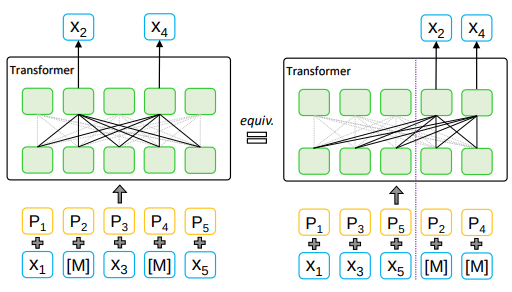
\includegraphics[keepaspectratio]{results/MLM.png}}

}

\caption{\label{fig-MLM}Concept de fonctionnement de MLM}

\end{figure}%

\textbf{Forces} :

Modèle robuste, encore largement utilisé comme baseline dans les
comparaisons.

Excellente capacité de contextualisation : le vecteur d'un mot varie
selon son usage dans la phrase.

Large éventail d'applications : classification, question-réponse,
reconnaissance d'entités nommées.

\textbf{Limites} :

Coût en calcul élevé : latence importante pour l'encodage, peu adapté
aux environnements contraints.

\begin{center}\rule{0.5\linewidth}{0.5pt}\end{center}

\subsection{2. MPNet (all-mpnet-base-v2)}\label{mpnet-all-mpnet-base-v2}

\textbf{Rappel} : XLNet comme étape intermédiaire

Avant MPNet, XLNet
(\textcite{yang2020xlnetgeneralizedautoregressivepretraining}) avait été
proposé pour surmonter une limite de BERT :

BERT prédit les tokens masqués indépendamment les uns des autres (Masked
Language Modeling).

XLNet introduit le Permuted Language Modeling (PLM), où l'ordre des
tokens est permuté et les prédictions s'effectuent de manière
auto-régressive.

Cela permet de capturer les dépendances entre tokens prédits, ce que
BERT ne faisait pas.

\begin{figure}

\centering{

\pandocbounded{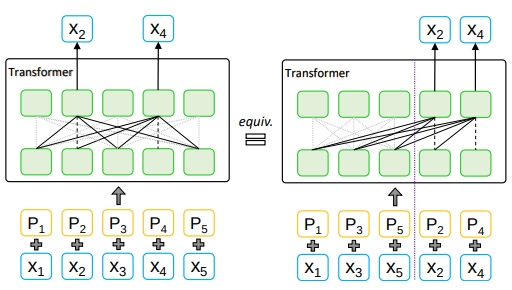
\includegraphics[keepaspectratio]{results/PLM.png}}

}

\caption{\label{fig-PLM}Concept de fonctionnement de PLM}

\end{figure}%

\textbf{Limite de XLNet} : comme l'ordre des tokens est modifié, le
modèle ne dispose pas toujours de la position exacte des mots dans leur
séquence originale. Cela crée un décalage entre le pré-entraînement
(phrases permutées) et l'utilisation réelle (phrases dans l'ordre
normal).

\textbf{Principes de MPNet}

MPNet (Masked and Permuted Pre-training for Language Understanding)
combine les avantages de BERT et XLNet :

Comme BERT, il conserve la visibilité complète du contexte grâce au
masquage (Masked Language Modeling).

Comme XLNet, il introduit des dépendances entre tokens prédits, en les
générant dans un ordre auto-régressif.

En plus, MPNet ajoute un mécanisme d'input consistency : le modèle
connaît la position exacte de chaque token, même ceux masqués, ce qui
corrige la limite de XLNet.
(\textcite{song2020mpnetmaskedpermutedpretraining})

\begin{figure}

\centering{

\pandocbounded{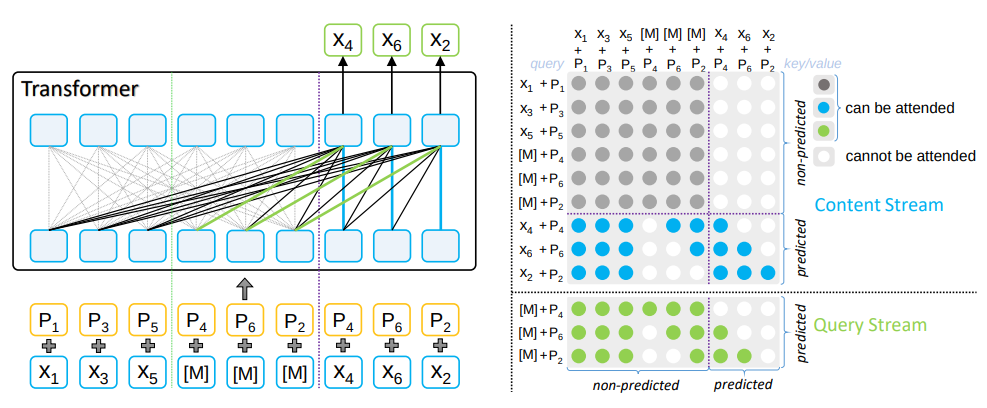
\includegraphics[keepaspectratio]{results/MPNET.png}}

}

\caption{\label{fig-MPNET}Concept de fonctionnement de MPNET}

\end{figure}%

\textbf{Forces}

Excellente précision sur les tâches de similarité sémantique et de
classification fine.

Combine le meilleur de BERT (vision contextuelle) et XLNet (dépendances
entre prédictions).

Recommandé pour les applications où la qualité des représentations est
critique (retrieval, recherche sémantique, Q\&A).

\textbf{Limites}

Plus coûteux que les modèles distillés comme MiniLM.

Temps d'inférence et mémoire encore relativement élevés.

\begin{center}\rule{0.5\linewidth}{0.5pt}\end{center}

\subsection{3. MiniLM / all-MiniLM-L6-v2}\label{minilm-all-minilm-l6-v2}

\textbf{Références clés} :

MiniLM (\textcite{wang2020minilm}) repose sur la distillation de
connaissances : un petit modèle (student) apprend à imiter les
distributions d'attention d'un modèle plus grand (teacher).

La variante all-MiniLM-L6-v2 est entraînée spécifiquement pour les
sentence embeddings, via un objectif contrastif sur de larges corpus.

\textbf{Forces} :

Rapidité et faible coût computationnel, adapté aux applications temps
réel ou aux environnements contraints.Latence très réduite, tout en
conservant une précision compétitive par rapport à des modèles plus
lourds.Bon choix pour le multilingue et les systèmes embarqués.

\textbf{Limites} :

Légère perte de performance (5-8\% en moyenne) par rapport à MPNet sur
des tâches de similarité ou de classification fine.Moins adapté pour des
textes longs ou des tâches nécessitant une compréhension très fine du
contexte.

\begin{center}\rule{0.5\linewidth}{0.5pt}\end{center}

\section{Méthodologie appliquée}\label{muxe9thodologie-appliquuxe9e}

\subsection{1. Données et
préparation}\label{donnuxe9es-et-pruxe9paration}

Un échantillon de 1 000 descriptions produits a été extrait de la base
nettoyée afin de limiter les coûts de calcul tout en gardant une
représentativité des catégories. Les données ont ensuite été divisées en
\textbf{train/test (80/20)} de manière stratifiée pour préserver la
distribution des classes.

\begin{center}\rule{0.5\linewidth}{0.5pt}\end{center}

\subsection{2. Encodage des textes}\label{encodage-des-textes}

Les descriptions ont été transformées en vecteurs denses à l'aide de la
librairie \textbf{Sentence Transformers (Hugging Face)}. Trois modèles
ont été comparés :

\begin{itemize}
\tightlist
\item
  \textbf{all-MiniLM-L6-v2} : léger, optimisé pour la rapidité,
\item
  \textbf{all-mpnet-base-v2} : plus coûteux mais plus précis,
\item
  \textbf{bert-base-uncased} : modèle historique, utilisé comme
  baseline.
\end{itemize}

Chaque encodage a été chronométré et sauvegardé afin d'assurer la
reproductibilité des expériences.

\begin{center}\rule{0.5\linewidth}{0.5pt}\end{center}

\subsection{3. Modélisation
supervisée}\label{moduxe9lisation-supervisuxe9e}

Pour évaluer la qualité des embeddings, un modèle de \textbf{régression
logistique} a été retenu comme classifieur de référence. Ce choix se
justifie par :

\begin{itemize}
\tightlist
\item
  sa simplicité d'entraînement,
\item
  sa rapidité d'exécution,
\item
  sa pertinence comme baseline pour comparer différentes
  représentations.
\end{itemize}

L'entraînement et l'évaluation ont été réalisés avec un modèle de
logistique regression.

\begin{center}\rule{0.5\linewidth}{0.5pt}\end{center}

\subsection{4. Évaluation et
comparaison}\label{uxe9valuation-et-comparaison}

Les performances ont été mesurées à l'aide des principales métriques de
classification (\textbf{F1-score, précision, rappel, accuracy}). En
parallèle, le \textbf{temps d'encodage} et le \textbf{temps de
prédiction} ont été suivis afin d'intégrer une dimension d'efficacité
computationnelle.

Les résultats de chaque combinaison \emph{embedding + classifieur} ont
ensuite été centralisés pour comparaison.

\begin{tcolorbox}[enhanced jigsaw, leftrule=.75mm, opacitybacktitle=0.6, titlerule=0mm, arc=.35mm, toprule=.15mm, breakable, toptitle=1mm, coltitle=black, colframe=quarto-callout-note-color-frame, bottomrule=.15mm, colback=white, colbacktitle=quarto-callout-note-color!10!white, opacityback=0, bottomtitle=1mm, title=\textcolor{quarto-callout-note-color}{\faInfo}\hspace{0.5em}{\emph{Pour rappel}}, left=2mm, rightrule=.15mm]

\textbf{Accuracy (Exactitude)} : Mesure le pourcentage total de
description correctement classifiées par le modèle parmi toutes les
images de l'ensemble de test. Elle donne une vue d'ensemble de la
performance globale du modèle.

\textbf{Précision (Precision)} : Mesure la proportion d'éléments
correctement identifiés comme appartenant à une classe spécifique parmi
tous ceux que le modèle a prédits comme appartenant à cette classe. Elle
permet d'évaluer la capacité du modèle à éviter les faux positifs.

\textbf{Rappel (Recall)} : Mesure la proportion d'éléments appartenant
réellement à une classe spécifique qui sont correctement identifiés par
le modèle. Elle évalue la capacité du modèle à détecter tous les
éléments pertinents pour une classe donnée.

\textbf{F1-score} : Représente la moyenne harmonique de la précision et
du rappel. Il offre une mesure équilibrée de la performance du modèle,
en tenant compte à la fois des faux positifs et des faux négatifs.

\textbf{Matrice de confusion} : Tableau qui détaille le nombre de
prédictions correctes et incorrectes pour chaque classe. Elle permet de
visualiser les erreurs du modèle et d'identifier les classes qui posent
problème.

\end{tcolorbox}

\begin{center}\rule{0.5\linewidth}{0.5pt}\end{center}

\section{Comparaison synthétique}\label{comparaison-synthuxe9tique}

Comparaison des modèles sur les données de test.

\begin{figure}

\begin{minipage}{0.50\linewidth}

\centering{

\pandocbounded{
\includegraphics[keepaspectratio]{results/fig_acc.png}}

}

\subcaption{\label{fig-scatter-plot}Compromis temps/performance en
fonction des embeddings}

\end{minipage}%
%
\begin{minipage}{0.50\linewidth}

\centering{

\pandocbounded{
\includegraphics[keepaspectratio]{results/fig_bar_time.png}}

}

\subcaption{\label{fig-bar-plot}Temps de calcul en fonction des
embeddings}

\end{minipage}%

\caption{\label{fig-embeddings-comparaison}Analyse des méthodes
d'embeddings}

\end{figure}%

\begin{figure}

\centering{

\pandocbounded{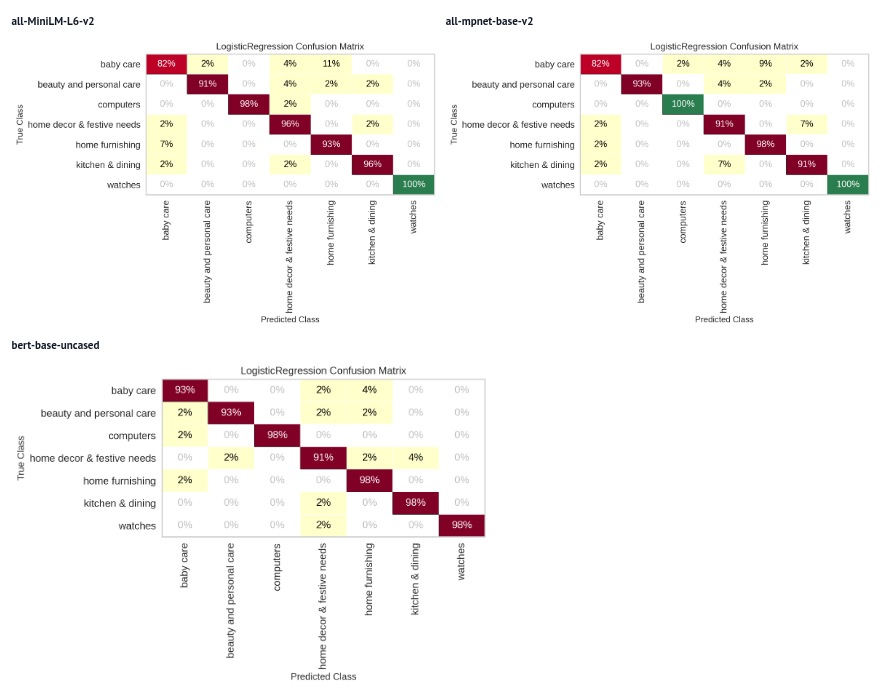
\includegraphics[keepaspectratio]{results/confusion_matrix.png}}

}

\caption{\label{fig-comparaison-confusion-matrix}Confusion matrix en
fonction de la méthode d'embedding utilisée.}

\end{figure}%

\begin{figure}

\centering{

\pandocbounded{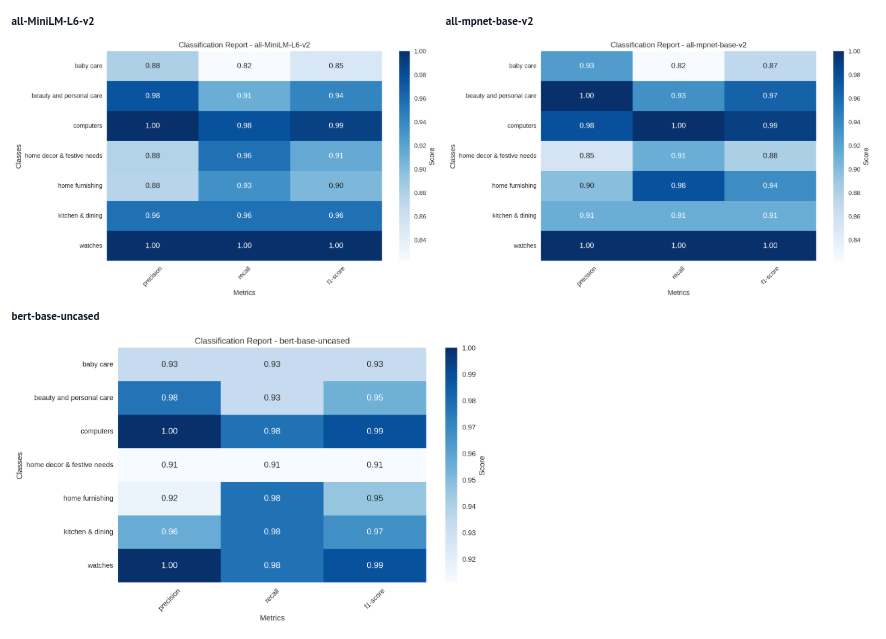
\includegraphics[keepaspectratio]{results/classification_reports.png}}

}

\caption{\label{fig-comparaison-class-report}Confusion matrix en
fonction de la méthode d'embedding utilisée.}

\end{figure}%

\section{Features importances globales et
locales}\label{features-importances-globales-et-locales}

L'analyse des features importances dans le cadre de modèles de
classification basés sur des embeddings de type Sentence Transformers
(vectorisés en 768 dimensions) pose une difficulté majeure :
l'interprétation des coefficients d'un modèle de régression logistique
devient complexe, car les dimensions latentes ne sont pas directement
interprétables par un humain. En effet, ces embeddings, bien
qu'efficaces pour capturer des relations sémantiques, masquent la
signification concrète des features sous-jacentes. Pour contourner cette
limite et obtenir des insights actionnables, j'ai complété l'analyse par
une étude des matrices de confusion. Celle-ci permet d'évaluer les
performances du modèle en identifiant les classes fréquemment
confondues, offrant ainsi une perspective complémentaire à
l'interprétation des features importances.''

\begin{figure}

\centering{

\pandocbounded{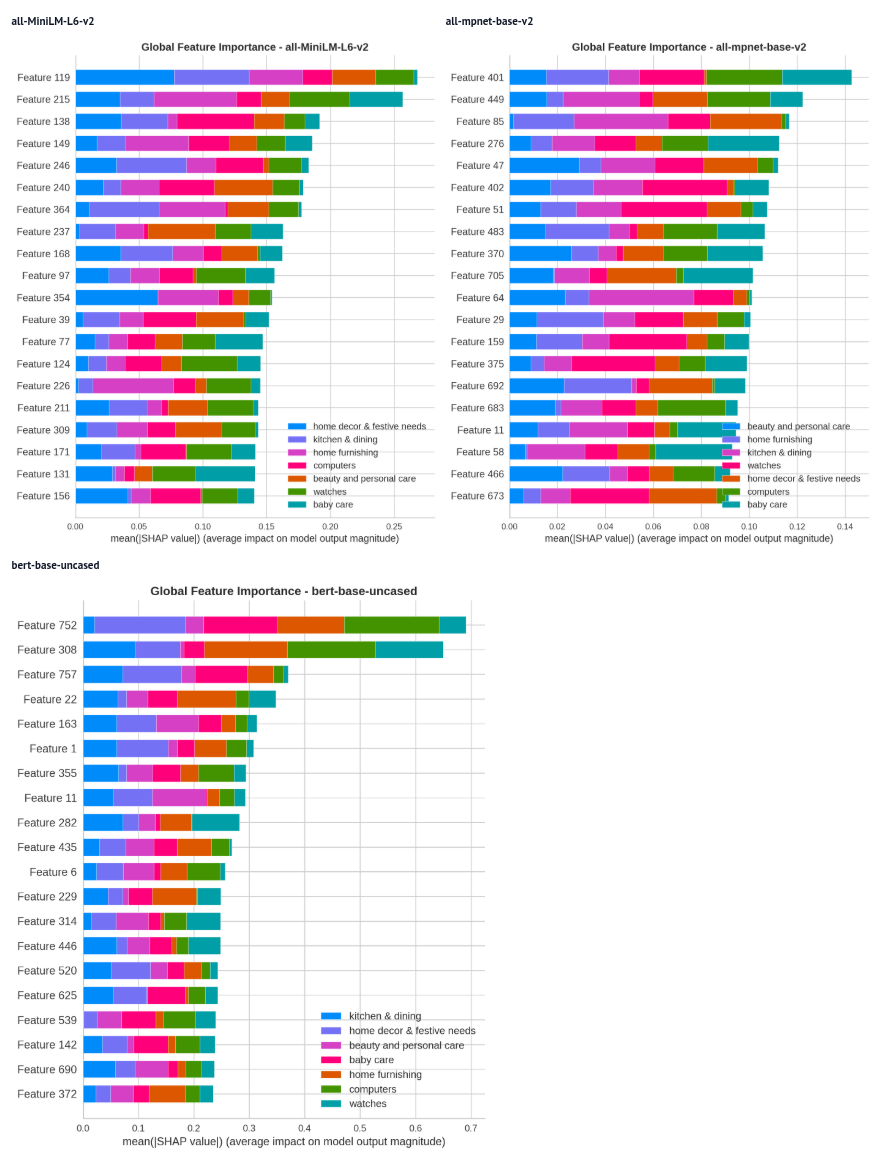
\includegraphics[keepaspectratio]{results/global_importances.png}}

}

\caption{\label{fig-comparaison-global-importance}Global features
importance en fonction de la méthode d'embedding utilisée.}

\end{figure}%

\begin{figure}

\centering{

\pandocbounded{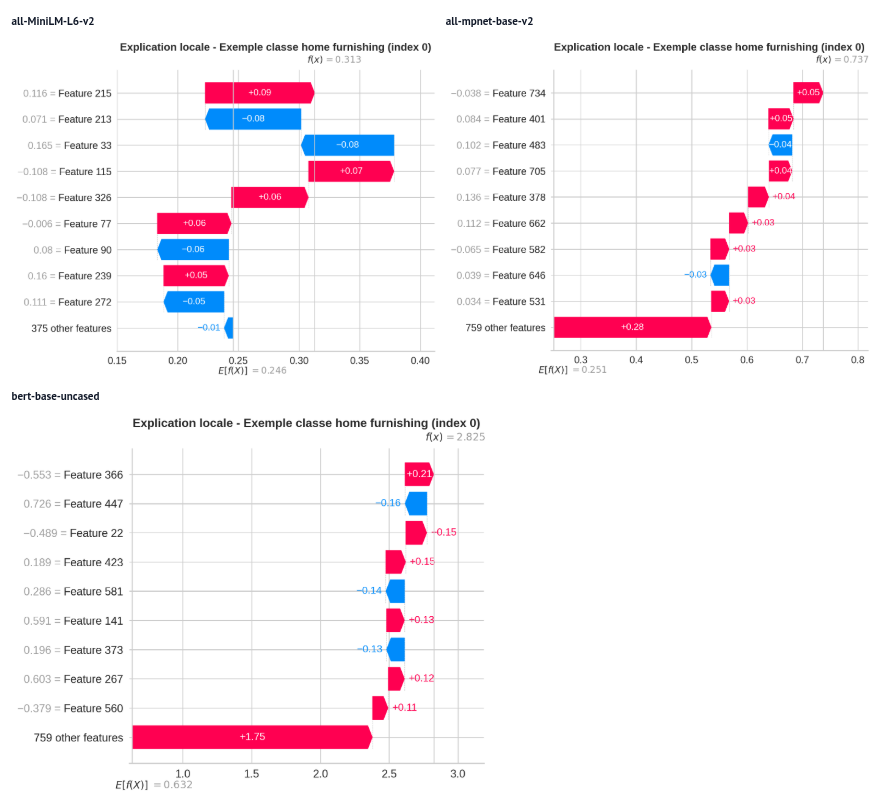
\includegraphics[keepaspectratio]{results/local_importances.png}}

}

\caption{\label{fig-comparaison-global-importance}Local features
importance en fonction de la méthode d'embedding utilisée.}

\end{figure}%

Les résultats de cette étude comparative montrent des différences
significatives entre les modèles d'embeddings testés, tant en
performance qu'en efficacité computationnelle. Parmi les trois modèles
évalués, \textbf{all-MiniLM-L6-v2} apparaît comme le meilleur compromis.

Il combine une performance stable sur l'ensemble des catégories (macro
F1-score 0.89, micro F1-score 0.91) avec un temps de calcul réduit
(\textasciitilde100 secondes pour le dataset testé). Ce modèle maintient
particulièrement bien ses performances sur les catégories
sous-représentées, ce qui se reflète dans son macro F1-score supérieur
aux autres modèles.

En comparaison, bert-base-uncased atteint un micro F1-score légèrement
supérieur (0.92), mais son coût computationnel est jusqu'à cinq fois
plus élevé, sans gain significatif sur les catégories critiques telles
que baby care ou beauty \& personal care. Quant à all-mpnet-base-v2, il
affiche une performance moyenne solide (macro F1-score 0.87) et se
distingue sur certaines catégories spécifiques, comme home decor \&
festive needs, où il obtient un F1-score parfait.

Ces résultats suggèrent que all-MiniLM-L6-v2 est le choix optimal pour
un équilibre entre rapidité et précision, tandis que bert-base-uncased
pourrait être envisagé lorsque la performance prime sur les contraintes
de temps, bien que le gain marginal ne justifie pas toujours le surcoût
computationnel.

\section{Limites et améliorations
possibles}\label{limites-et-amuxe9liorations-possibles}

La méthodologie présentée comporte plusieurs limites :

\begin{itemize}
\tightlist
\item
  \textbf{Taille du jeu de données} : l'échantillon utilisé (1 000
  descriptions) permet de réduire les temps de calcul, mais il reste
  restreint. Les résultats obtenus ne sont donc pas nécessairement
  généralisables à un corpus de plus grande ampleur.
\item
  \textbf{Modèle de classification simple} : l'utilisation d'une
  régression logistique constitue un bon point de départ pour comparer
  des embeddings, mais elle ne reflète pas le potentiel maximal des
  représentations, qui pourraient mieux s'exprimer avec des modèles plus
  complexes (p.~ex. réseaux de neurones légers ou gradient boosting).
\item
  \textbf{Diversité des données} : les descriptions analysées
  appartiennent à un domaine particulier (produits). Les performances
  des modèles pourraient varier sur d'autres types de textes (avis
  clients, articles techniques, etc.).
\end{itemize}

\subsection{Pistes d'amélioration}\label{pistes-damuxe9lioration}

\begin{itemize}
\tightlist
\item
  Étendre l'expérimentation à un corpus plus large afin de vérifier la
  robustesse des résultats.
\item
  Évaluer d'autres classifieurs supervisés (Random Forest, XGBoost, MLP)
  pour tester la sensibilité des embeddings aux choix de modèles.
\item
  Explorer des approches multilingues ou spécialisées par domaine (ex.
  modèles d'embeddings entraînés sur du texte produit/retail).
\end{itemize}

\begin{center}\rule{0.5\linewidth}{0.5pt}\end{center}

\textbf{En conclusion} :

\begin{itemize}
\item
  \textbf{Pour une application nécessitant rapidité et légèreté} :
  all-MiniLM-L6-v2 est le meilleur choix pour des utilisation limitées
  en puissance de calcul.
\item
  \textbf{Pour une application critique en précision} :
  all-mpnet-base-v2 est recommandé, avec des benchmarks solides en
  retrieval et classification.
\item
  \textbf{Pour du fine-tuning sur un domaine spécifique} : BERT base
  uncased reste une référence, avec une abondance de travaux récents
  confirmant sa robustesse après adaptation.
\end{itemize}


\printbibliography[title=References]



\end{document}
